Im folgenden Abschnitt~\ref{subsec:der-originale-plan} wird zunächst der originale Plan erläutert und in Einzelschritten dargestellt, warum dieser so nicht implementiert wurde.
Daraufhin folgt in Abschnitt~\ref{subsec:randomized-depth-first-search} eine generelle Beschreibung des allgemeinen \qq{Randomised-Depth-First-Search} Algorithmus.
Zum Schluss ist in Abschnitt~\ref{subsec:unsere-implementierung} erklärt, wie wir diesen Algorithmus zur Labyrinth-Generation implementiert haben.
\subsection{Der originale Plan}\label{subsec:der-originale-plan}
Vor der Detailbeschreibung zunächst einmal die grobe Idee.
Von einem bestimmten Punkt aus geht das Programm einen Schritt in eine zufällige Richtung, bis es das Ziel in der Mitte erreicht hat.
Danach soll noch einmal durch den nun erstellten Zielpfad gelaufen werden, und an zufälligen Stellen Abzweigungen vom Hauptpfad generiert werden.
Im Detail würde dies erreicht werden, indem wir eine zwei dimensionale Liste mit Weg-Objekten erstellen, einen Start aufrufen, und dieser sich zufällig eine Richtung als Attribut einstellt und Koordinaten für das nächste Objekt zurückgibt.
Sobald alle Wege fertig sind, sollte noch einmal über alle iteriert werden, und je nachdem, ob sie eine Richtung haben, entweder eine 0 (Wand) oder eine 1 (Weg) in einen zwei dimensionalen Bit-Array eingetragen werden.

Zwar kommen einige dieser Punkte schon nah an unsere finale Implementierung, jedoch kann man auf den ersten Blick schon einige Probleme finden. Wenn zuerst über zufällige Richtungen NUR der Zielpfad generiert wird, und später erst die Sackgassen, kann es schnell passieren, dass der Zielpfad sich \qq{einschneckt}, also sich selbst in eine Ecke läuft, aus der er nicht mehr entkommen kann, da er nicht zweimal über dasselbe Feld laufen darf. (Siehe Abbildung~\ref{fig:einschnecken})
    \begin{figure}[ht!]
    \centering
                \begin{tikzpicture}[node distance={30mm}, main/.style = {draw, circle,outer sep=0pt}]
                \tikzstyle{rand} = [node distance={30mm}, rand/.style = {draw, circle,outer sep=0pt}]
                \tikzstyle{klrand} = [node distance={15mm}, klrand/.style = {draw, circle,outer sep=0pt}]
                \tikzstyle{klw} = [node distance={13mm}, klw/.style = {draw, circle,outer sep=0pt}]
                    \node[rand] (a) { };
                    \node[rand] (b) [below of=a] { };
                    \node[rand] (c) [right of=b] { };
                    \node[rand] (d) [above of=c] { };
                    \node[klrand] (e) [left of=d] { };
                    \node[klrand] (f) [below of=e] { };
                    \node[klw] (g) [right of=f] { };
                    \node[node distance={13mm}] (h) [above of=g] { };
                    \node[node distance={10mm}] (i) [left of=h] { };
                    \node[node distance={10mm}] (j) [below of=i] { };
                    \node[node distance={9mm}] (k) [right of=j] { };

                    \draw (a) to (b);
                    \draw (b) to (c);
                    \draw (c) to (d);
                    \draw (d) to (e);
                    \draw (e) to (a);
                    \draw (e) to (f);
                    \draw (f) to (g);
                    \draw (g) to (h);
                    \draw (h) to (i);
                    \draw (i) to (j);
                    \draw (j) to (k);

                \end{tikzpicture}

        \caption{Einschneckung}
        \label{fig:einschnecken}
    \end{figure}

Also müsste man unter großen Aufwand einen Vorrechner erstellen, der solche Einschränkungen verhindert.
Zudem kann es hier auch passieren, dass das Ziel selbst umzingelt wird. Auch der Fakt, dass im Nachhinein ein zusätzlicher Durchlauf für die Sackgassen erfolgen sollte, ist extrem suboptimal.

Aus diesen Gründen wurde die Idee verworfen und es wurde beim Überlegen systematischer vorgegangen. Anstatt das Rad neu zu erfinden, haben wir uns damit beschäftigt, an welchen schon existierenden Algorithmen man sich orientieren kann.
Da einige innerhalb des Teams sich schon vorher mit Algorithmen beschäftigt hatten, kam recht schnell der Entschluss dazu \qq{Randomised-Depth-First-Search} als unseren Orientierung-Punkt zu verwenden.
Und was \qq{Randomised-Depth-First-Search} genau ist, und wie es implementiert wurde, wird in den nun folgenden Abschnitten behandelt.



\subsection{Randomized-Depth-First-Search}\label{subsec:randomized-depth-first-search}
    \begin{figure}[ht!]
        \centering
        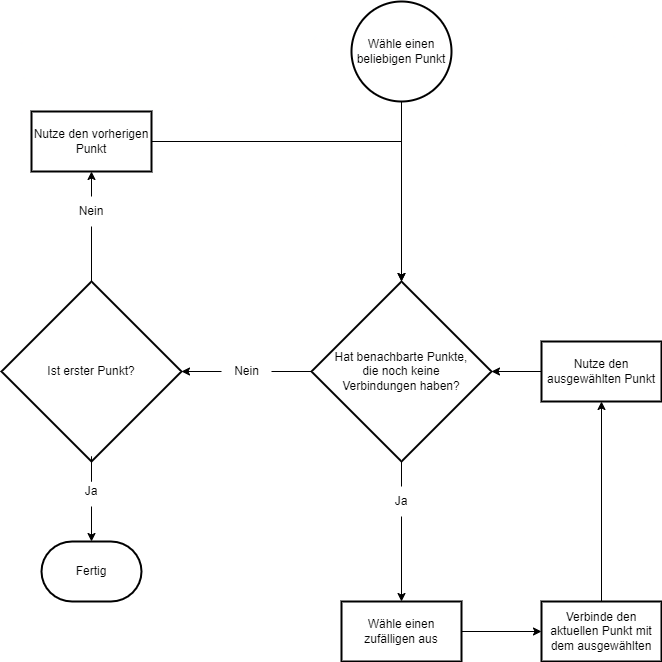
\includegraphics[width=\paperwidth/2]{../assets/img/Randomised-Depth-First-Search}
        \caption{Randomized-Depth-First-Search Ablauf}
        \label{fig:randomized-depth-first-search-flow}
    \end{figure}
Gegeben ist ein Feld der Breite $w$ und Höhe $h$.
Das Feld beinhaltet alle Punkte $p\in\{(x,y)\in\mathbb{N}^2, 0\leq x<w, 0\leq y<h\}$.
Daraus wird zunächst ein beliebiger Startpunkt ausgewählt.
Die benachbarten Punkte werden nach Punkten durchsucht, die noch keine Verbindungen haben.
Der Startpunkt wird zufällig mit einem dieser Punkte verbunden.
Anschließend wird der Verbindungspunkt zum neuen Startpunkt.
Hat der Startpunkt keine benachbarten Punkte ohne Verbindungen, so wird der vorherige Startpunkt überprüft.
Dies wird wiederholt, bis es keinen Punkt mehr gibt, der keine Verbindung hat.
Der Ablauf ist auch in Abbildung~\ref{fig:randomized-depth-first-search-flow} dargestellt.

\subsection{Unsere Implementierung}\label{subsec:unsere-implementierung}
    \begin{figure*}[ht!]
        \lstinputlisting[label={lst:randomised-depth-first-search-code}, caption={Randomized-Depth-First-Search Implementierung}, language=java]{../assets/code/recursive_randomised_depth_first_search.java}
    \end{figure*}
Wir haben uns für den \qq{Randomised-Depth-First-Search} Algorithmus entschieden, da dieser in einer guten Laufzeit von $\Theta(n)$\footnote{Im worst-- sowie bestcase braucht der Algorithmus $n\cdot x+h$ Sekunden, wobei $n$ die Anzahl der Felder ist und $x,h\in\mathbb{R}^+$.} hat und subjektiv schöne Abzweigungen generiert.


Zunächst haben wir eine rekursive Implementierung gewählt.
Dies ist zwar bei der Beschreibung des Algorithmus intuitiver, wollen wir jedoch große Labyrinthe generieren, so kann es zu einer StackOverflowException kommen, weshalb auch noch eine iterative Implementierung geplant ist.

Als Datenmodell dient uns ein ungerichteter Graph.
Graphen sind eine Ansammlung von Knoten, die über Kanten miteinander verbunden sind.
(Siehe Abbildung~\ref{fig:what-is-a-graph})
Knoten haben einen Wert und Kanten setzen diese in Relation.
Ungerichtet heißt dabei, dass die Verbindung in beide Richtungen gilt.

    \begin{figure}[ht!]
        \centering
        \begin{tabular}{l c}
            Liste &
            \begin{minipage}{0.7\textwidth}
                \centering
                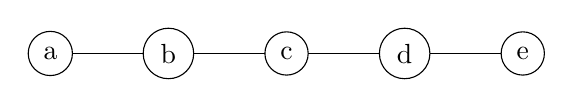
\begin{tikzpicture}[node distance={15mm}, main/.style = {draw, circle,outer sep=0pt}]
                    \node[main] (a) {a};
                    \node[main] (b) [right of=a] {b};
                    \node[main] (c) [right of=b] {c};
                    \node[main] (d) [right of=c] {d};
                    \node[main] (e) [right of=d] {e};

                    \draw (a) to (b);
                    \draw (b) to (c);
                    \draw (c) to (d);
                    \draw (d) to (e);

                    \title{Liste}
                \end{tikzpicture}
            \end{minipage}\\
            \vspace{15mm}\\
            Baum &
            \begin{minipage}{0.7\textwidth}
                \centering
                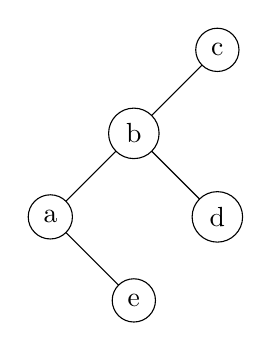
\begin{tikzpicture}[node distance={15mm}, main/.style = {draw, circle,outer sep=0pt}]
                    \node[main] (a) {a};
                    \node[main] (b) [above right of=a] {b};
                    \node[main] (c) [above right of=b] {c};
                    \node[main] (d) [below right of=b] {d};
                    \node[main] (e) [below right of=a] {e};

                    \draw (a) to (b);
                    \draw (b) to (c);
                    \draw (b) to (d);
                    \draw (a) to (e);


                    \title{Baum}
                \end{tikzpicture}
            \end{minipage}\\
            \vspace{15mm}\\
            Graph &
            \begin{minipage}{0.7\textwidth}
                \centering
                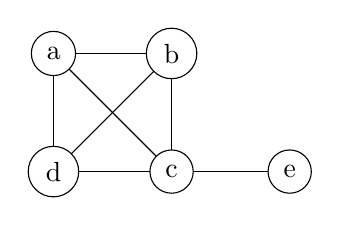
\begin{tikzpicture}[node distance={15mm}, main/.style = {draw, circle,outer sep=0pt}]
                    \node[main] (a) {a};
                    \node[main] (b) [right of=a] {b};
                    \node[main] (c) [below of=b] {c};
                    \node[main] (d) [left of=c] {d};
                    \node[main] (e) [right of=c] {e};

                    \draw (a) to (b);
                    \draw (b) to (c);
                    \draw (c) to (d);
                    \draw (d) to (a);
                    \draw (a) to (c);
                    \draw (b) to (d);
                    \draw (c) to (e);

                    \title{Graph}
                \end{tikzpicture}
            \end{minipage}
        \end{tabular}

        \caption{Was ist ein Graph?}
        \label{fig:what-is-a-graph}
    \end{figure}
In unserem Fall ist der Wert die Koordinate als Punkt $p\in\{(x,y)\in\mathbb{N}^2, 0\leq x<w, 0\leq y<h\}$.
Da die Dimensionen bekannt sind, ist die Menge aller Punkte $P$ abzählbar (eine endliche Menge).
Dies gestaltet die Implementierung einfach, da so nur die Kanten gespeichert werden müssen.

Mit diesen Voraussetzungen fangen wir nun in Code~\ref{lst:randomised-depth-first-search-code} mit einem Startpunkt \lstinline{current} an und lassen uns so lange alle anliegenden Knoten ohne Verbindung ausgeben, bis es keine mehr gibt.
Mit einem zufälligen dieser Punkte aus \lstinline{adjacent} wird jetzt fortgefahren.
Auf unserem Graphen verbinden wir die Knoten an den beiden Punkten.
Danach wird die gegebene Methode rekursiv erneut aufgerufen, dieses Mal mit dem ausgewählten Punkt.
